% ============================================================
\chapter{Dynamical Systems --- Definitions and Examples}
\label{ch:definitions}
% ============================================================

In 1889, Henri Poincar\'e entered a competition organized by King Oscar II of
Sweden: prove the stability of the solar system. Not only did Poincar\'e fail
to prove stability, but he discovered something far more profound: the
existence of behaviors so complicated that any long-term prediction becomes
impossible. This is where dynamical systems theory was born: the study of
how the states of a system evolve over time, with all the richness --- order,
chaos, bifurcations --- that this entails.

% ------------------------------------------------------------
\section{Introduction}
% ------------------------------------------------------------

A dynamical system is a mathematical model describing the temporal evolution
of a state in a given space. This evolution may be governed by a differential
equation (continuous time) or by an iterated map (discrete time). In this
chapter, we lay down the fundamental definitions and illustrate these concepts
through classical examples from physics, biology, and engineering.

\section{Continuous Dynamical Systems}

\begin{definition}[Autonomous continuous dynamical system]
An \textbf{autonomous continuous dynamical system} on an open set
$U \subseteq \R^n$ is defined by the ordinary differential equation
\[
    \dot{x} = f(x), \qquad x \in U,
\]
where $f : U \to \R^n$ is a vector field of at least class $C^1$.
\end{definition}

\begin{definition}[Non-autonomous system]
A \textbf{non-autonomous dynamical system} has the form
\[
    \dot{x} = f(t, x), \qquad (t, x) \in \R \times U,
\]
where $f$ depends explicitly on time $t$.
\end{definition}

\begin{remark}
Any non-autonomous system $\dot{x} = f(t,x)$ on $\R^n$ can be transformed
into an autonomous system on $\R^{n+1}$ by setting $\dot{t} = 1$, yielding
the augmented system:
\[
    \begin{pmatrix} \dot{x} \\ \dot{t} \end{pmatrix} =
    \begin{pmatrix} f(t,x) \\ 1 \end{pmatrix}.
\]
\end{remark}

\subsection{Existence and Uniqueness of Solutions}

\begin{theorem}[Picard-Lindel\"of / Cauchy-Lipschitz]
\label{thm:picard-lindelof}
Let $f : U \to \R^n$ be locally Lipschitz on the open set $U \subseteq \R^n$.
For every $x_0 \in U$, there exists a maximal interval
$I(x_0) = (\alpha, \omega)$ with $-\infty \leq \alpha < 0 < \omega \leq +\infty$
and a unique maximal solution $\varphi(\cdot, x_0) : I(x_0) \to U$ of the
initial value problem
\[
    \dot{x} = f(x), \qquad x(0) = x_0.
\]
\end{theorem}

\begin{proof}
The classical proof uses the Banach fixed-point theorem applied to the
Picard operator
\[
    (T\varphi)(t) = x_0 + \int_0^t f(\varphi(s))\, ds
\]
in the space $C([0,h], \overline{B}(x_0, r))$ equipped with the uniform norm,
for $h > 0$ sufficiently small. The Lipschitz condition
$\norm{f(x) - f(y)} \leq L\norm{x - y}$ ensures that $T$ is a contraction
for $h < 1/L$. Uniqueness on the maximal interval follows from the
extension theorem and Gr\"onwall's lemma.
\end{proof}

\begin{theorem}[Behavior at boundaries of the maximal interval]
\label{thm:blowup}
Let $\varphi(\cdot, x_0) : (\alpha, \omega) \to U$ be the maximal solution.
If $\omega < +\infty$, then for every compact set $K \subseteq U$, there
exists $t_K < \omega$ such that $\varphi(t, x_0) \notin K$ for all $t > t_K$.
In other words, the trajectory ``blows up'' or leaves every compact set in
finite time.
\end{theorem}

\section{Flows and Semi-flows}

\begin{definition}[Flow]
The \textbf{flow} associated with the system $\dot{x} = f(x)$ is the map
\[
    \varphi : \mathcal{D} \subseteq \R \times U \to U, \qquad
    (t, x_0) \mapsto \varphi(t, x_0) = \varphi_t(x_0),
\]
where $\mathcal{D}$ is the maximal open domain of definition. The flow
satisfies:
\begin{enumerate}
    \item $\varphi_0 = \mathrm{Id}_U$ (initial condition);
    \item $\varphi_{t+s} = \varphi_t \circ \varphi_s$ for all admissible
    $s, t$ (group property).
\end{enumerate}
\end{definition}

\begin{proposition}[Regularity of the flow]
If $f \in C^k(U, \R^n)$ with $k \geq 1$, then the flow
$\varphi : \mathcal{D} \to U$ is of class $C^k$ in $(t, x_0)$.
\end{proposition}

\begin{definition}[Semi-flow]
A \textbf{semi-flow} is defined for $t \geq 0$ only. It satisfies the same
properties as the flow, but only for $t, s \geq 0$. Parabolic partial
differential equations naturally generate semi-flows.
\end{definition}

\section{Orbits, Trajectories, and Limit Sets}

\begin{definition}[Orbit]
The \textbf{orbit} (or \textbf{trajectory}) through $x_0$ is the set
\[
    \gamma(x_0) = \{\varphi(t, x_0) : t \in I(x_0)\} \subseteq U.
\]
The \textbf{positive orbit} is $\gamma^+(x_0) = \{\varphi(t, x_0) : t \geq 0\}$
and the \textbf{negative orbit} is $\gamma^-(x_0) = \{\varphi(t, x_0) : t \leq 0\}$.
\end{definition}

\begin{definition}[Equilibrium points]
A point $x^* \in U$ is an \textbf{equilibrium point} (or \textbf{fixed point},
\textbf{stationary point}) of the system $\dot{x} = f(x)$ if $f(x^*) = 0$.
Equivalently, $\varphi(t, x^*) = x^*$ for all $t$.
\end{definition}

\begin{definition}[Periodic orbit]
An orbit $\gamma(x_0)$ is \textbf{periodic} if there exists $T > 0$ such that
$\varphi(T, x_0) = x_0$ and $\varphi(t, x_0) \neq x_0$ for $0 < t < T$.
The smallest such $T$ is called the \textbf{minimal period}.
\end{definition}

\begin{definition}[$\omega$-limit set]
The \textbf{$\omega$-limit set} of $x_0$ is
\[
    \omega(x_0) = \bigcap_{T \geq 0} \overline{\{\varphi(t, x_0) : t \geq T\}}.
\]
A point $y$ belongs to $\omega(x_0)$ if and only if there exists a sequence
$t_n \to +\infty$ such that $\varphi(t_n, x_0) \to y$.
\end{definition}

\begin{definition}[$\alpha$-limit set]
Analogously, the \textbf{$\alpha$-limit set} is
\[
    \alpha(x_0) = \bigcap_{T \leq 0} \overline{\{\varphi(t, x_0) : t \leq T\}}.
\]
\end{definition}

\begin{proposition}[Properties of limit sets]
\label{prop:omega-props}
Let $\gamma^+(x_0)$ be bounded. Then:
\begin{enumerate}
    \item $\omega(x_0)$ is nonempty, compact, and connected;
    \item $\omega(x_0)$ is invariant under the flow: $\varphi_t(\omega(x_0)) = \omega(x_0)$ for all $t$;
    \item $\mathrm{dist}(\varphi(t, x_0), \omega(x_0)) \to 0$ as $t \to +\infty$.
\end{enumerate}
\end{proposition}

\section{Phase Space and Phase Portrait}

\begin{definition}[Phase portrait]
The \textbf{phase portrait} of a dynamical system is the partition of the
phase space $U$ into orbits. It provides a global qualitative description
of the dynamics.
\end{definition}

\begin{remark}
Two distinct orbits cannot cross (a consequence of the uniqueness of
solutions). The phase space is therefore partitioned into disjoint orbits.
\end{remark}

\begin{example}[Simple harmonic oscillator]
Consider the simple harmonic oscillator
\[
    \ddot{q} + \omega^2 q = 0,
\]
written as a first-order system with $x_1 = q$, $x_2 = \dot{q}$:
\[
    \begin{cases}
        \dot{x}_1 = x_2, \\
        \dot{x}_2 = -\omega^2 x_1.
    \end{cases}
\]
The system matrix is $A = \begin{pmatrix} 0 & 1 \\ -\omega^2 & 0 \end{pmatrix}$,
with eigenvalues $\lambda = \pm i\omega$. The orbits are ellipses centered
at the origin. The phase portrait is a \textbf{center}.
\end{example}

\begin{example}[Simple pendulum]
\label{ex:pendulum}
The undamped simple pendulum satisfies
\[
    \ddot{\theta} + \frac{g}{l}\sin\theta = 0.
\]
Setting $x_1 = \theta$, $x_2 = \dot{\theta}$:
\[
    \begin{cases}
        \dot{x}_1 = x_2, \\
        \dot{x}_2 = -\frac{g}{l}\sin x_1.
    \end{cases}
\]
The equilibrium points are $(\theta^*, 0)$ with $\theta^* = k\pi$, $k \in \Z$.
Points $\theta^* = 2k\pi$ are centers (downward positions) and points
$\theta^* = (2k+1)\pi$ are saddles (upward positions).
\end{example}

\begin{intuition}
The phase portrait of the pendulum reveals two types of motion:
\begin{itemize}
    \item Closed trajectories near centers correspond to oscillations
    (librations);
    \item Open trajectories far from centers correspond to full rotations
    of the pendulum.
\end{itemize}
The trajectories separating these two regions are the \textbf{separatrices},
which connect the saddle points.
\end{intuition}

% --- Phase portrait of the pendulum ---
\begin{center}
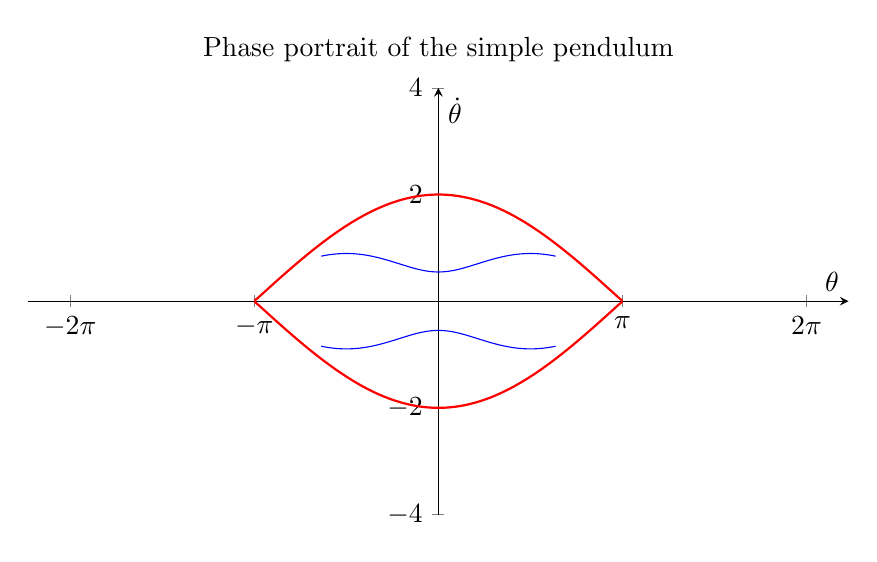
\begin{tikzpicture}
    \begin{axis}[
        width=12cm, height=7cm,
        xlabel={$\theta$}, ylabel={$\dot{\theta}$},
        xmin=-7, xmax=7, ymin=-4, ymax=4,
        axis lines=middle,
        xtick={-6.283,-3.14159,0,3.14159,6.283},
        xticklabels={$-2\pi$,$-\pi$,$0$,$\pi$,$2\pi$},
        title={Phase portrait of the simple pendulum}
    ]
    % Separatrices
    \addplot[thick, red, domain=-3.14:3.14, samples=100]
        {sqrt(2*(1+cos(deg(x))))};
    \addplot[thick, red, domain=-3.14:3.14, samples=100]
        {-sqrt(2*(1+cos(deg(x))))};
    % Small oscillations
    \addplot[blue, domain=-2:2, samples=80]
        {sqrt(0.5*(1-cos(deg(2*x)))/2 + 0.3)};
    \addplot[blue, domain=-2:2, samples=80]
        {-sqrt(0.5*(1-cos(deg(2*x)))/2 + 0.3)};
    \end{axis}
\end{tikzpicture}
\end{center}

\section{Discrete Dynamical Systems}

\begin{definition}[Discrete dynamical system]
A \textbf{discrete dynamical system} is defined by the iteration of a map
$f : U \to U$:
\[
    x_{n+1} = f(x_n), \qquad n \in \N.
\]
The orbit of $x_0$ is the sequence $(x_0, f(x_0), f^2(x_0), \ldots)$
where $f^n = \underbrace{f \circ f \circ \cdots \circ f}_{n \text{ times}}$.
\end{definition}

\begin{definition}[Fixed and periodic points]
A point $x^*$ is a \textbf{fixed point} of $f$ if $f(x^*) = x^*$.
A point $x^*$ is \textbf{periodic of period} $p$ if $f^p(x^*) = x^*$
and $f^k(x^*) \neq x^*$ for $1 \leq k < p$.
\end{definition}

\begin{example}[Logistic map]
The \textbf{logistic map} is defined by
\[
    f_r(x) = rx(1-x), \qquad x \in [0,1], \quad r \in [0,4].
\]
The fixed points satisfy $x = rx(1-x)$, giving $x^* = 0$ and
$x^* = 1 - 1/r$ (for $r > 1$).
\end{example}

\section{First Integrals and Conservative Systems}

\begin{definition}[First integral]
A function $H : U \to \R$ of class $C^1$ is a \textbf{first integral}
(or \textbf{constant of motion}) of the system $\dot{x} = f(x)$ if $H$ is
constant along every orbit:
\[
    \frac{d}{dt} H(\varphi(t, x_0)) = \nabla H(\varphi(t, x_0)) \cdot
    f(\varphi(t, x_0)) = 0 \quad \forall t.
\]
\end{definition}

\begin{theorem}[Dimensional reduction]
If $H$ is a first integral such that $\nabla H(x) \neq 0$ on a level set
$\Sigma_c = \{x \in U : H(x) = c\}$, then $\Sigma_c$ is an $(n-1)$-dimensional
submanifold invariant under the flow. The dynamics thus reduces to the study
of a system on $\Sigma_c$.
\end{theorem}

\begin{definition}[Hamiltonian system]
A \textbf{Hamiltonian system} on $\R^{2n}$ is defined by
\[
    \dot{q}_i = \frac{\partial H}{\partial p_i}, \qquad
    \dot{p}_i = -\frac{\partial H}{\partial q_i}, \qquad i = 1, \ldots, n,
\]
where $H : \R^{2n} \to \R$ is the \textbf{Hamiltonian function} (energy).
The Hamiltonian $H$ is automatically a first integral.
\end{definition}

\begin{example}[Pendulum as a Hamiltonian system]
The simple pendulum (Example~\ref{ex:pendulum}) is Hamiltonian with
\[
    H(\theta, p) = \frac{p^2}{2} - \frac{g}{l}\cos\theta,
\]
where $p = \dot{\theta}$. The level curves of $H$ coincide with the orbits
of the phase portrait.
\end{example}

\section{Dissipative Systems and Liouville's Volume}

\begin{theorem}[Liouville's formula]
\label{thm:liouville}
Let $\Omega(t) = \varphi_t(\Omega_0)$ be the image of a measurable domain
$\Omega_0 \subseteq U$ under the flow. Then
\[
    \frac{d}{dt}\mathrm{Vol}(\Omega(t)) = \int_{\Omega(t)} \mathrm{div}\, f(x)\, dx.
\]
\end{theorem}

\begin{corollary}
If $\mathrm{div}\, f(x) = 0$ for all $x \in U$, the flow preserves volume
(\textbf{incompressible} system). This holds for every Hamiltonian system.
\end{corollary}

\begin{definition}[Dissipative system]
A system is \textbf{dissipative} if $\mathrm{div}\, f(x) < 0$ on $U$.
In this case, volumes in phase space contract over time.
\end{definition}

\begin{example}[Damped oscillator]
The damped harmonic oscillator
\[
    \dot{x}_1 = x_2, \qquad \dot{x}_2 = -\omega^2 x_1 - 2\gamma x_2, \quad \gamma > 0,
\]
has divergence $\mathrm{div}\, f = -2\gamma < 0$. It is a dissipative system.
Volumes contract at the rate $e^{-2\gamma t}$.
\end{example}

\section{Famous Dynamical Systems}

\begin{example}[Lotka-Volterra system]
The Lotka-Volterra predator-prey model is
\[
    \dot{x} = \alpha x - \beta xy, \qquad \dot{y} = \delta xy - \gamma y,
\]
with $\alpha, \beta, \gamma, \delta > 0$. The nontrivial equilibrium point is
$(\gamma/\delta, \alpha/\beta)$. This system possesses the first integral
$H(x,y) = \delta x - \gamma \ln x + \beta y - \alpha \ln y$.
\end{example}

\begin{example}[Lorenz system]
The Lorenz system, introduced in 1963, is
\[
    \dot{x} = \sigma(y - x), \qquad
    \dot{y} = \rho x - y - xz, \qquad
    \dot{z} = xy - \beta z,
\]
with classical parameter values $\sigma = 10$, $\rho = 28$, $\beta = 8/3$.
The divergence is $\mathrm{div}\, f = -\sigma - 1 - \beta < 0$:
the system is dissipative.
\end{example}

\begin{codeblock}[title=\textbf{Simulation of the Lorenz system}]
\begin{minted}{python}
import numpy as np
from scipy.integrate import solve_ivp
import matplotlib.pyplot as plt

def lorenz(t, state, sigma=10, rho=28, beta=8/3):
    x, y, z = state
    return [sigma*(y - x), rho*x - y - x*z, x*y - beta*z]

sol = solve_ivp(lorenz, [0, 50], [1, 1, 1], max_step=0.01,
                dense_output=True)
t = np.linspace(0, 50, 10000)
xyz = sol.sol(t)

fig = plt.figure(figsize=(10, 7))
ax = fig.add_subplot(111, projection='3d')
ax.plot(xyz[0], xyz[1], xyz[2], lw=0.5, color='steelblue')
ax.set_xlabel('x'); ax.set_ylabel('y'); ax.set_zlabel('z')
ax.set_title("Lorenz Attractor")
plt.tight_layout()
plt.savefig("lorenz_attractor.pdf")
plt.show()
\end{minted}
\end{codeblock}

\section{Topological Equivalence and Conjugacy}

\begin{definition}[Topological equivalence]
Two dynamical systems $\dot{x} = f(x)$ and $\dot{y} = g(y)$ are
\textbf{topologically equivalent} if there exists a homeomorphism
$h : U \to V$ that maps orbits of $f$ to orbits of $g$ while preserving
orientation (direction of traversal).
\end{definition}

\begin{definition}[Topological conjugacy]
Two systems are \textbf{topologically conjugate} if the change of variable
$h$ also respects the time parameterization:
$h \circ \varphi_t^f = \varphi_t^g \circ h$ for all $t$.
\end{definition}

\begin{remark}
Topological conjugacy is stronger than topological equivalence. Conjugacy
preserves the periods of periodic orbits, unlike mere equivalence.
\end{remark}

\section{Exercises}

\begin{exercise}[Equilibrium points]
Find all equilibrium points of the system
\[
    \dot{x} = y - x^2, \qquad \dot{y} = x - 2.
\]
Determine the nature of each equilibrium point by computing the Jacobian
matrix and its eigenvalues.
\end{exercise}

\begin{exercise}[First integral]
Show that $H(x, y) = x^2 + y^2 - 2\ln(1 + x^2 + y^2)$ is a first integral
of the system
\[
    \dot{x} = -y\,\frac{x^2 + y^2}{1 + x^2 + y^2}, \qquad
    \dot{y} = x\,\frac{x^2 + y^2}{1 + x^2 + y^2}.
\]
\end{exercise}

\begin{exercise}[Explicit flow]
Compute explicitly the flow of the linear system $\dot{x} = Ax$ with
$A = \begin{pmatrix} 0 & 1 \\ -1 & 0 \end{pmatrix}$.
Verify the group property $\varphi_{t+s} = \varphi_t \circ \varphi_s$.
\end{exercise}

\begin{exercise}[Dissipative system]
Compute the divergence of the R\"ossler system
\[
    \dot{x} = -y - z, \qquad \dot{y} = x + ay, \qquad \dot{z} = b + z(x - c),
\]
and determine for which parameter values $a, b, c$ the system is dissipative.
\end{exercise}

\begin{exercise}[Logistic map]
For the logistic map $f_r(x) = rx(1-x)$:
\begin{enumerate}
    \item Find the fixed points and study their stability as a function of $r$.
    \item Find the period-2 orbits and study their stability.
    \item Show that for $r > 4$, the orbit of almost every initial point in
    $[0,1]$ escapes to $-\infty$.
\end{enumerate}
\end{exercise}

\begin{exercise}[Volume and Liouville]
Consider the system $\dot{x} = f(x)$ on $\R^3$ with
$f(x,y,z) = (y, -x - \epsilon y, z - \epsilon z^3)$.
\begin{enumerate}
    \item Compute $\mathrm{div}\, f$.
    \item For which values of $\epsilon$ is the system dissipative?
    Conservative?
    \item Qualitatively describe the behavior of volumes over time.
\end{enumerate}
\end{exercise}
